% ════════════════════════════════════════════════════════════════════════════
% BiCA Benchmark Paper — v1 Draft
% Target: Journal of Chemical Information and Modeling (ACS)
% Style: ACS two-column preprint
% ════════════════════════════════════════════════════════════════════════════

\documentclass[11pt,twocolumn]{article}

\usepackage[T1]{fontenc}
\usepackage[utf8]{inputenc}
\usepackage[margin=2cm]{geometry}
\usepackage{microtype}
\usepackage{amsmath,amssymb}
\usepackage{graphicx}
\usepackage{booktabs}
\usepackage{multirow}
\usepackage{tabularx}
\usepackage[table]{xcolor}
\usepackage[colorlinks=true,linkcolor=blue,citecolor=blue,urlcolor=blue]{hyperref}
\usepackage{cleveref}
\usepackage{natbib}
\usepackage{authblk}
\usepackage{abstract}
\usepackage{titlesec}
\usepackage{parskip}

% ── Colours for tables ────────────────────────────────────────────────────────
\definecolor{best}{RGB}{209,236,191}   % light green — best in group
\definecolor{good}{RGB}{255,243,205}   % light yellow
\definecolor{poor}{RGB}{255,220,215}   % light red

% ── Title formatting ─────────────────────────────────────────────────────────
\titleformat{\section}{\large\bfseries}{\thesection}{1em}{}
\titleformat{\subsection}{\normalsize\bfseries}{\thesubsection}{1em}{}
\titleformat{\subsubsection}{\normalsize\itshape}{\thesubsubsection}{1em}{}

% ── Metadata ─────────────────────────────────────────────────────────────────
\title{\textbf{Systematic Benchmarking of Sequence-Based Protein--Ligand Binding
       Affinity Prediction: When Do Cross-Attention Models Outperform
       Gradient-Boosted Trees, and What Residues Do They Learn?}}

\author[1]{[Author 1]}
\author[2]{[Author 2]}
\affil[1]{[Institution 1]}
\affil[2]{[Institution 2]}

\date{}

% ── Keywords macro ────────────────────────────────────────────────────────────
\newcommand{\keywords}[1]{\noindent\textit{Keywords:} #1\vspace{1em}}

% ════════════════════════════════════════════════════════════════════════════

\begin{document}

\maketitle

\keywords{binding affinity prediction; cross-attention; protein--ligand
  interaction; interpretability; benchmark; drug--target affinity;
  ESM-2; ChemBERTa}

% ── Abstract ─────────────────────────────────────────────────────────────────
\begin{abstract}
Predicting protein--ligand binding affinity from sequence data is central to
structure-free drug discovery.  Despite hundreds of published deep learning
architectures, practitioners still frequently reach for gradient-boosted
trees on molecular fingerprints, yet systematic comparisons that hold
evaluation protocol constant are rare.  We present a comprehensive benchmark
of 313 experiments spanning 12 model families---from amino-acid composition
features and ECFP fingerprints up to per-residue ESM-2 protein embeddings
and per-token ChemBERTa-77M ligand embeddings---evaluated on the
BindingDB\_filtered dataset (24,700 records, Bemis--Murcko scaffold split)
with multi-seed stability analysis.  Our key finding is quantitative: a
Random Forest using ECFP4 fingerprints and amino-acid composition achieves
test RMSE~$=1.007$ and Pearson~$r=0.747$, which no sequence-only deep
learning model we tested surpassed.  Among deep learning models, our novel
Bidirectional Cross-Attention (BiCA~v2) architecture---operating on
per-residue ESM-2 embeddings and per-token ChemBERTa-2 embeddings---achieves
test RMSE~$=1.108 \pm 0.037$ across three seeds and, uniquely, produces
interpretable residue$\times$token attribution maps.  Applying Integrated
Gradients and value-weighted attention to 149 inhibitors of the same
kinase-like protein, BiCA~v2 identifies a single cysteine (C463 in the
C-lobe context \texttt{ERPEGCPEKVY}) as the dominant binding-relevant residue
(AttentionPool weight~$= 0.949$, $485\times$ above uniform), consistent with
known covalent inhibitor pharmacology of ABL1-family kinases.  This
convergence of two independent attribution methods (attention and gradients)
on a chemically sensible residue demonstrates that BiCA~v2 learns
mechanistically interpretable representations without structural supervision.
We provide all 313 trained models, reproducible evaluation code, and a
public leaderboard to accelerate fair comparison in this field.
\end{abstract}

% ════════════════════════════════════════════════════════════════════════════
\section{Introduction}
% ════════════════════════════════════════════════════════════════════════════

Accurate prediction of protein--ligand binding affinity is a central
objective in computational drug discovery.  Strong binding affinity ($K_d$,
$K_i$, or $IC_{50}$) is necessary but not sufficient for a compound to
become a drug; nevertheless, the ability to rank millions of candidate
molecules by predicted affinity before synthesis dramatically accelerates
hit identification and lead optimisation.

Early computational approaches relied on physics-based scoring functions
embedded in molecular docking programs, which require three-dimensional
structural data.  The scarcity of protein crystal structures for many
therapeutically relevant targets has motivated development of
\emph{sequence-only} methods that infer binding affinity directly from
primary sequences of the protein and the SMILES string of the ligand.
BindingDB~\cite{liu2007bindingdb,gilson2016bindingdb,chen2024bindingdb2024},
now containing over 2.9 million binding measurements, provides the substrate
for training such models at scale.

A first wave of deep learning methods represented proteins as character
sequences fed to convolutional or recurrent networks, and ligands as SMILES
strings encoded similarly.  DeepDTA~\cite{ozturk2018deepdta} demonstrated
that two parallel CNN encoders could match or exceed classical fingerprint
methods on the KIBA and Davis benchmarks.  Graph-neural-network
variants~\cite{nguyen2021graphdta} subsequently improved performance by
encoding ligands as molecular graphs, preserving atom-level topology.
Cross-modal attention mechanisms---allowing protein residues to directly
``attend'' to ligand atoms---emerged as a natural inductive bias for capturing
binding-site specificity, and models such as
MolTrans~\cite{huang2021moltrans} introduced attention to this domain.

A second wave exploited pre-trained language models.  Protein language models
such as ESM-2~\cite{lin2023esm2}, trained on hundreds of millions of
evolutionary sequences, encode rich structural and functional information in
per-residue embeddings without solving the folding problem.  Similarly,
chemical language models such as ChemBERTa-2~\cite{ahmad2022chemberta2},
pre-trained on 77~million SMILES strings from PubChem, produce per-token
embeddings that capture sub-structural chemical context.  The natural
hypothesis is that applying cross-attention \emph{directly} between
per-residue protein tokens and per-atom ligand tokens---rather than pooling
either into a fixed vector first---would allow the model to discover binding
site geometry implicitly.

The most recent high-water mark in this paradigm is
PSICHIC~\cite{tran2024psichic}, which incorporates physicochemical
constraints into a graph neural network operating on sequence data and
achieves near structure-based accuracy.  However, systematic comparisons
that (i) hold the train--test split constant across all models, (ii) evaluate
over multiple random seeds, and (iii) cover the full landscape from classical
baselines to modern language-model hybrids are still rare.  Without such
comparisons it is difficult to assess whether deep learning truly provides a
meaningful advantage over mature tree ensembles at typical drug-discovery
dataset sizes.

We make four contributions:
\begin{enumerate}
  \item \textbf{Comprehensive benchmark}: 313 experiments across 12 model
    families (ridge, random forest, XGBoost, LightGBM, CNN, LSTM,
    transformer-seq, flat transformer, GCN, GAT, BiCA~v1, BiCA~v2) on a
    common scaffold split with identical featurisation pipeline.

  \item \textbf{BiCA~v2 architecture}: A novel Bidirectional Cross-Attention
    model that operates on true per-residue ESM-2 tokens and per-token
    ChemBERTa-2 embeddings, employing stacked bidirectional cross-attention
    layers followed by learned attention pooling.

  \item \textbf{Multi-seed stability analysis}: Three-seed evaluation of the
    best BiCA~v2 configuration reveals scaffold-dependent variance and
    quantifies the honest gap to the RF baseline ($\Delta\text{RMSE}
    = 0.064$).

  \item \textbf{Biological validation of interpretability}: Per-compound
    consensus attribution (Integrated Gradients $\times$ AttentionPool)
    identifies a single cysteine in the ABL1 kinase C-lobe as the dominant
    binding-relevant residue across 149 compounds---without structural
    supervision.
\end{enumerate}

% ════════════════════════════════════════════════════════════════════════════
\section{Methods}
% ════════════════════════════════════════════════════════════════════════════

\subsection{Dataset and Preprocessing}

We used the \textbf{BindingDB\_filtered} split from the publicly available
BALM benchmark~\cite{balm2025jcim} hosted on HuggingFace
(\texttt{BALM/BALM-benchmark}, configuration \texttt{BindingDB\_filtered}).
After merging all provided splits and de-duplicating protein--SMILES pairs,
the dataset contains 24,700~records.  The binding affinity label $Y$ is
$-\log_{10}(K_d/\text{M})$ (pKd), a continuous value that correlates
linearly with binding free energy.

Sequences were truncated to a maximum of 1200~amino acids and 512~SMILES
characters prior to featurisation.  No additional preprocessing (e.g.,
protonation or tautomer standardisation) was applied to preserve the
benchmark's reproducibility.

\subsection{Data Splitting}

A single, shared \textbf{Bemis--Murcko scaffold split}~\cite{bemis1996scaffolds}
was applied with random seed~42, yielding 70\,\%~training (17,290~records),
10\,\%~validation (2,470~records), and 20\,\%~test (4,940~records) sets.
Molecules sharing an identical Murcko framework were assigned to the same
partition, ensuring that test-set scaffolds were unseen during training.

For multi-seed stability analysis we additionally evaluated the best
configurations at seeds~$\{42, 123, 456\}$, which induce different scaffold
partitions and quantify variance attributable to test-set difficulty.

\subsection{Ligand Representations}

\paragraph{Fingerprint-based.}
ECFP4 (Morgan radius~2, 1024~bits)~\cite{rogers2010ecfp} and ECFP6
(radius~3, 1024~bits) were computed via RDKit.  MACCS-167~keys,
RDKit~200~2D descriptors, and one-hot SMILES character encodings were also
evaluated.

\paragraph{Pre-trained ligand embeddings.}
ChemBERTa-2 models were loaded from HuggingFace in three sizes:
\texttt{ChemBERTa-5M-MTR} (mean-pooled, $d=600$),
\texttt{ChemBERTa-77M-MTR} (mean-pooled and per-token,
$d=384$)~\cite{ahmad2022chemberta2}, and
\texttt{ChemBERTa-100M-MLM} (mean-pooled, $d=768$).
Mean-pooled embeddings were used with tree and flat MLP models; per-token
embeddings (preserving the full sequence of ChemBERTa sub-word tokens,
maximum length~126 after stripping \texttt{[CLS]}/\texttt{[SEP]}) were used
exclusively with BiCA~v2.

\subsection{Protein Representations}

\paragraph{Composition-based.}
Amino-acid composition (AAC,~$d=20$), dipeptide composition ($d=400$), and
$k$-mer frequencies ($k=3$, $d=8000$) were computed from the raw sequence.

\paragraph{Pre-trained protein embeddings.}
ESM-2~\cite{lin2023esm2} was used in four sizes: 8M~parameters
($d=320$), 35M~($d=480$), 150M~($d=640$), and 650M~($d=1280$).
For tree and flat MLP models, mean-pooled representations were used.
For BiCA~v2, per-residue embeddings were used (padded and masked up to
512~residues; embeddings stored in \texttt{float16} to halve disk usage).
ProtT5-XL~\cite{elnaggar2021prottrans} (\texttt{prot\_electra\_256})
and ESMc-300M were also evaluated in selected configurations.

\subsection{Model Architectures}

\subsubsection{Baseline Models}
Ridge regression, Random Forest (RF)~\cite{breiman2001rf},
XGBoost~\cite{chen2016xgboost}, and LightGBM~\cite{ke2017lightgbm} were
fitted to concatenated ligand--protein feature vectors.  RF used 500~trees
with no constraint on tree depth; XGBoost and LightGBM used 1000 estimators
with learning rate~0.05.

\subsubsection{Sequence Models}
One-dimensional CNNs, bidirectional LSTMs, and sequence transformers were
trained on character/BPE tokenisations of SMILES and protein sequences.
For LSTM, BPE vocabularies of 512 and 1000 tokens were compared against
atom-level and character-level tokenisations.  For transformer-seq, a
four-layer, eight-head transformer was applied independently to each modality
before concatenation.

\subsubsection{Graph Neural Network Models}
GCN~\cite{kipf2017gcn} and GAT~\cite{velickovic2018gat} models encoded
ligands as RDKit atom-feature graphs (node features: atom type, charge,
hybridisation, aromaticity; edge features: bond type).  Protein embeddings
were provided as a fixed vector (mean-pooled from the selected PLM).

\subsubsection{BiCA v1 (Flat Cross-Attention)}
The original BiCA~v1 model applied bidirectional cross-attention between
mean-pooled, projected protein and ligand vectors.  With mean-pooled inputs,
each modality reduces to a single token, so cross-attention degenerates to
a learned bilinear interaction.  BiCA~v1 was included as an architectural
control to isolate the benefit of true per-residue attention.

\subsubsection{BiCA v2 (True Sequence Cross-Attention)}
\label{sec:bica_v2}

BiCA~v2 is the central novel model.  The architecture is:

\paragraph{Input projections.}
Per-residue ESM-2 embeddings $\mathbf{P} \in \mathbb{R}^{B \times L_p \times d_p}$ and per-token ChemBERTa embeddings $\mathbf{L} \in \mathbb{R}^{B \times L_l \times d_l}$ are linearly projected to a shared hidden dimension $h=256$ and normalised:
\[
  \mathbf{H}_p = \text{LayerNorm}(W_p \mathbf{P}), \quad
  \mathbf{H}_l = \text{LayerNorm}(W_l \mathbf{L}).
\]

\paragraph{Bidirectional cross-attention layers.}
Two stacked bidirectional cross-attention blocks are applied.  Each block
performs Pre-LN cross-attention in both directions simultaneously:
\begin{align}
  \mathbf{H}_p^{(t+1)} &= \mathbf{H}_p^{(t)} + \text{DropPath}(\text{MHA}(\text{LN}(\mathbf{H}_p^{(t)}),\; \text{LN}(\mathbf{H}_l^{(t)}))) \\
  \mathbf{H}_l^{(t+1)} &= \mathbf{H}_l^{(t)} + \text{DropPath}(\text{MHA}(\text{LN}(\mathbf{H}_l^{(t)}),\; \text{LN}(\mathbf{H}_p^{(t)})))
\end{align}
Each MHA block uses $N_h=8$ heads.  A position-wise feed-forward network
(FFN, GELU activation, $4h$ inner dimension) follows each attention
sub-layer.  Stochastic depth (DropPath) with linearly increasing rate
$[0, 0.1]$ is applied to residual streams.

\paragraph{Attention pooling.}
After the final cross-attention layer, each sequence is reduced to a fixed
vector by a learned gated-attention pooler:
\[
  \boldsymbol{s} = \sum_{i} w_i \mathbf{H}_i, \quad
  w_i = \frac{\exp(f(\mathbf{H}_i))}{\sum_j \exp(f(\mathbf{H}_j))},
\]
where $f(\cdot)$ is a single linear layer.  Padding positions receive
$-\infty$ before softmax.

\paragraph{Predictor.}
Pooled protein and ligand vectors are independently processed by
GELU~+~dropout projection layers, concatenated, and fed to a three-layer MLP
with LayerNorm and GELU activations, producing a scalar prediction.

Total trainable parameters: 3.94~million.

\subsubsection{Training Details}
All deep learning models were trained with AdamW (learning rate
$5 \times 10^{-4}$, weight decay $10^{-4}$), batch size~128, maximum
100~epochs, with early stopping after 20~epochs without validation RMSE
improvement.  A single NVIDIA GPU was used throughout.  All models were
implemented in PyTorch~\cite{paszke2019pytorch}; pre-trained embeddings
were loaded via HuggingFace Transformers~\cite{wolf2020transformers}.

\subsection{Evaluation Protocol}

\paragraph{Primary metric.}
Root mean square error (RMSE) on the held-out test set.

\paragraph{Secondary metrics.}
Pearson's $r$ and Spearman's $\rho$ between predicted and true pKd.

\paragraph{Multi-seed analysis.}
For the best BiCA~v2 configuration
(\texttt{bica\_v2\_chemberta77M\_tokens}), three independent scaffold splits
(seeds~$\{42, 123, 456\}$) were evaluated.  Seed-to-seed variance in RMSE
reflects both model stochasticity and variation in test-scaffold difficulty.

\subsection{Interpretability Methods}

\subsubsection{Attention Source Taxonomy}

BiCA~v2 exposes four complementary attribution signals:
\begin{itemize}
  \item \textbf{S1}: Cross-attention $p\to l$ weights
    $\mathbf{A}^{(p2l)} \in \mathbb{R}^{B \times H \times L_p \times L_l}$
    from the last layer.  Summing over ligand positions gives per-residue
    ``outgoing attention''.
  \item \textbf{S2}: Cross-attention $l\to p$ weights
    $\mathbf{A}^{(l2p)} \in \mathbb{R}^{B \times H \times L_l \times L_p}$.
    Summing over ligand positions gives per-residue ``incoming attention''.
  \item \textbf{S3}: AttentionPool protein weights
    $\mathbf{w}_p \in \mathbb{R}^{B \times L_p}$.  Directly controls the
    contribution of each residue to the prediction vector.
  \item \textbf{S4}: AttentionPool ligand weights
    $\mathbf{w}_l \in \mathbb{R}^{B \times L_l}$.
\end{itemize}

\subsubsection{Value-Weighted Attention}

Raw softmax attention weights $A_{ij}$ may be large for positions carrying
little information (``attention sinks'' analogous to \texttt{[CLS]} tokens in
BERT).  We correct for this by scaling each weight by the $\ell_2$~norm of
the corresponding Value vector:
\begin{equation}
  \tilde{A}_{ij} \propto A_{ij} \cdot \|\mathbf{v}_j\|_2,
\end{equation}
then re-normalising each row.  $\mathbf{v}_j$ is computed from the Value
projection $W_V$ of the cross-attention module applied to the (normalised)
source sequence.

\subsubsection{Integrated Gradients}

For each compound--protein pair, Integrated Gradients
(IG)~\cite{sundararajan2017ig} were computed via
Captum~\cite{kokhlikyan2020captum} on the post-projection, pre-attention
protein embedding $\mathbf{H}_p \in \mathbb{R}^{L_p \times h}$, using a
zero-vector baseline ($n_\text{steps}=50$).  Per-residue attribution is
defined as
\begin{equation}
  \alpha_i = \|\text{IG}(\mathbf{H}_p)_i\|_2,
\end{equation}
normalised to sum to~1.

\subsubsection{Consensus Attribution}

A consensus map combining IG and AttentionPool:
\begin{equation}
  c_i = \alpha_i^{(\text{IG})} \cdot w_i^{(\text{S3})},
\end{equation}
highlights residues that are simultaneously (a)~important according to
gradient-based attribution and (b)~heavily weighted by the pooling gate.
Residues with high $c_i$ are identified as ``persistent hot spots'' across
compounds.

\subsubsection{Per-Compound Experiment}

To test whether attribution is compound-specific or protein-dominated, we
selected the protein with the largest number of test-set compounds (1130
amino acids, 149~compounds, pKd range~$5.02$--$8.80$) and ran the complete
attribution pipeline for each compound individually.  ChemBERTa tokens were
decoded back to SMILES substrings via the \texttt{DeepChem/ChemBERTa-77M-MTR}
tokeniser to label the X-axis of residue$\times$token attention heatmaps.

% ════════════════════════════════════════════════════════════════════════════
\section{Results}
% ════════════════════════════════════════════════════════════════════════════

\subsection{Overall Benchmark: 12 Model Families on BindingDB}
\label{sec:overall}

\Cref{tab:leaderboard} summarises the best-performing configuration within
each model family.  The complete leaderboard of 313~experiments is provided in
\textbf{Supporting Information Table~S1}.

\begin{table}[htbp]
\centering
\caption{Best test-set performance per model family on the BindingDB\_filtered
  scaffold-split benchmark (seed~42).  RMSE lower is better; Pearson~$r$ and
  Spearman~$\rho$ higher is better.}
\label{tab:leaderboard}
\small
\begin{tabularx}{\linewidth}{lXrrrrr}
\toprule
Family & Best Configuration & RMSE$\downarrow$ & $r$$\uparrow$ & $\rho$$\uparrow$ & Train (s) \\
\midrule
\rowcolor{best}
Trees (RF)      & \texttt{rf\_ecfp4\_aac}           & 1.0065 & 0.747 & 0.674 & 23 \\
Trees (XGB)     & \texttt{xgb\_chemberta5M\_esm2\_650M}  & 1.0434 & 0.724 & 0.648 & 12 \\
Trees (LightGBM)& \texttt{lgbm\_ecfp4\_aac}         & 1.0528 & 0.720 & 0.640 & 6  \\
\rowcolor{good}
MLP (flat)      & \texttt{mlp\_chemberta100M\_esm2\_650M} & 1.1007 & 0.703 & 0.623 & 36 \\
BiCA v2         & \texttt{bica\_v2\_chemberta77M\_tokens} & 1.1080 & 0.703 & 0.625 & 54 \\
BiCA v1         & \texttt{bica\_chemberta5M\_esmc300M}    & 1.1020 & 0.702 & 0.631 & 45 \\
DistMat-CNN     & \texttt{distmat\_cnn\_esm2\_35M}        & 1.1092 & 0.697 & 0.631 & 1330 \\
LSTM            & \texttt{lstm\_smiles\_bpe1000\_prot\_bpe1000} & 1.1456 & 0.660 & 0.581 & 1083 \\
Flat transformer& \texttt{transformer\_chemberta100M\_electra} & 1.1194 & 0.679 & 0.602 & 78 \\
\rowcolor{poor}
TransformerSeq  & \texttt{transformer\_seq\_smiles\_atom} & 1.2096 & 0.606 & 0.514 & 647 \\
GAT             & \texttt{gat\_mol\_graph\_esm2\_650M}    & 1.1939 & 0.643 & 0.584 & 151 \\
GCN             & \texttt{gcn\_mol\_graph\_esm2\_35M}     & 1.2024 & 0.616 & 0.550 & 74  \\
Ridge           & \texttt{ridge\_chemberta5M\_esm2\_35M}  & 1.2544 & 0.595 & 0.526 & 0.2 \\
\bottomrule
\end{tabularx}
\end{table}

The most striking finding is that a Random Forest using 1024-bit ECFP4
fingerprints concatenated with 20-dimensional amino-acid composition (AAC)
achieves RMSE~$=1.007$ and Pearson~$r=0.747$---the best result across all
313~experiments---despite its trivial computational cost (23~seconds training
time on a single CPU core).  The best deep learning model, BiCA~v2 at
RMSE~$=1.108$, is $\Delta\text{RMSE}=0.10$ behind RF under seed~42.

Strikingly, adding more expressive protein representations does not
consistently help even for tree models: XGB with ESM-2-650M
embeddings (RMSE~$=1.043$) performs worse than RF with AAC (RMSE~$=1.007$),
suggesting that the AAC descriptor captures sufficient amino-acid-level
signal at this dataset scale.

\subsection{Representation and Architecture Ablations}

\paragraph{Protein representation.}
\Cref{tab:protein_ablation} shows that ESM-2 model size has limited impact
across the $8\text{M}$--$650\text{M}$ range: BiCA~v2 trained with
ESM-2-35M~($d=480$) achieves RMSE~$=1.108$ vs.~$1.143$ with ESM-2-150M,
suggesting that the cross-attention bottleneck---not protein embedding
capacity---limits performance at 17\,k training examples.

\paragraph{Ligand representation.}
Comparing mean-pooled ChemBERTa-5M ($d=600$) to per-token
ChemBERTa-77M~MTR ($d=384$) in BiCA~v2 (RMSE~$=1.102$ vs.~$1.108$) shows
similar performance, indicating that per-token chemical context provides
comparable signal to a larger mean-pooled embedding.

\paragraph{BiCA~v2 cross-attention heads.}
We observed anti-correlation between the S1 ($p\to l$) and S2 ($l\to p$)
attention sources across all test-set compounds (Pearson~$r=-0.83$ between
mean S1 and S2 per-residue profiles), indicating that the two attention
directions learn complementary, non-redundant views of the interaction.
This validates the bidirectional design as more than a symmetric duplicate.

\paragraph{Tokenisation strategy.}
In LSTM and TransformerSeq models, atom-level tokenisation consistently
outperforms BPE and character encodings (mean RMSE~$1.188$ vs.~$1.211$
for BPE-512 vs.~$1.234$ for character-level), confirming that chemical
substructure boundaries are more informative than learned byte-pair subwords
for SMILES.

\begin{table}[htbp]
\centering
\caption{Effect of protein representation on BiCA~v2 performance (seed~42).}
\label{tab:protein_ablation}
\small
\begin{tabular}{lcccc}
\toprule
Protein repr. & $d_p$ & RMSE$\downarrow$ & $r$$\uparrow$ \\
\midrule
ESM-2 35M  & 480  & \textbf{1.108} & \textbf{0.703} \\
ESM-2 150M & 640  & 1.143          & 0.680          \\
ESM-2 650M & 1280 & 1.156          & 0.662          \\
ProtElectra & 256 & 1.230          & 0.585          \\
\bottomrule
\end{tabular}
\end{table}

\subsection{Multi-Seed Stability of BiCA~v2}

Single-seed evaluation is insufficient to characterise deep learning
performance on scaffold splits, because different seed values yield different
scaffold difficulty distributions in the test set.  \Cref{tab:multiseed}
shows the three-seed evaluation of the best BiCA~v2 configuration.

\begin{table}[htbp]
\centering
\caption{Multi-seed evaluation of best BiCA~v2 and RF configurations.
  ``Test difficulty'' is the median pKd variance of test-set scaffolds;
  seed~456 draws an easier test set.}
\label{tab:multiseed}
\small
\begin{tabular}{lcccc}
\toprule
Model & Seed & Val RMSE & Test RMSE & Test $r$ \\
\midrule
\multirow{3}{*}{BiCA~v2} & 42  & 1.087 & 1.124 & 0.701 \\
                          & 123 & 1.082 & 1.135 & 0.698 \\
                          & 456 & 1.093 & 1.065 & 0.713 \\
\cmidrule{2-5}
& \textit{mean~$\pm$~sd} & $1.087\pm0.006$ & $1.108\pm0.037$ & $0.704\pm0.008$ \\
\midrule
\multirow{3}{*}{RF (ECFP4+AAC)} & 42  & -- & 1.007 & 0.747 \\
                                  & 123 & -- & 1.037 & 0.731 \\
                                  & 456 & -- & 1.089 & 0.702 \\
\cmidrule{2-5}
& \textit{mean~$\pm$~sd} & -- & $1.044\pm0.035$ & $0.727\pm0.023$ \\
\bottomrule
\end{tabular}
\end{table}

The honest RF--BiCA~v2 gap under matched scaffold splits is
$\Delta\text{RMSE} = 0.064$ (seed-averaged), smaller than the single-seed
figure of $0.101$ often cited in our preliminary analyses.  Seed~456
produces an easier test-scaffold distribution (lower mean scaffold pKd
variance), explaining the apparent RMSE improvement to~1.065 under that
seed.  The stability of BiCA~v2 (sd~$=0.037$) is comparable to RF
(sd~$=0.035$), confirming reproducibility.

\subsection{Per-Compound Interpretability of BiCA~v2}
\label{sec:interpret}

\subsubsection{AttentionPool Concentrates on a Single Cysteine Residue}

\Cref{fig:protein_consensus} shows the mean attribution profile across 149
test-set compounds binding to a 1130-residue kinase-like protein (truncated
to 512~residues by our featurisation protocol).  The S3~AttentionPool signal
is dominated by a single residue: \textbf{position~463} carries mean weight
$w_{463} = 0.949$, equivalent to $485\times$ the uniform expectation.  The
next-highest position~(127) receives weight $0.011$~($5.5\times$).

Decoding position~463 from the protein sequence gives the dipeptide context
\texttt{ERPEG\underline{C}PEKVY} (C-lobe region of the kinase domain).  The
underlined cysteine is consistent with a known reactive cysteine in the
C-lobe of ABL1-family kinases~\cite{nagar2002abl1structure,schindler2000abl1}.
Cysteine residues in solvent-accessible positions of kinase C-lobes are
known targets for covalent irreversible inhibitors; the BindingDB data for
this protein include several nanomolar compounds with confirmed covalent
mechanisms.  BiCA~v2 has learned to identify this residue without any
structural input.

\subsubsection{Value-Weighted Attention Eliminates Sink Tokens}

Raw cross-attention (S1) shows moderate focusing around several positions
but also places weight on a small set of ligand tokens irrespective of
compound identity---a pattern consistent with ``attention sink'' behaviour
analogous to \texttt{[CLS]} tokens in BERT-family models.  After applying
value-weighted correction (\Cref{sec:methods_vwa}), the spurious sink
contributions are suppressed and compound-specific residue--token
interactions emerge (\Cref{fig:vw_comparison}).

\subsubsection{Integrated Gradients Agree with AttentionPool on Top Residues}

The IG attribution profile (\Cref{fig:protein_consensus}, bottom panel) is
more distributed than S3~AttentionPool, with secondary peaks at positions
68, 79, 127, and~323 alongside the primary peak at~463.  The consensus
attribution (IG~$\times$~S3) highlights five persistent hot spots:
positions~\{68, 79, 127, 323, 463\}.  This convergence of two mechanistically
independent attribution methods (gradient propagation and attention weighting)
on the same residues substantiates that BiCA~v2 has learned genuine
binding-relevant representations.

The anti-correlation between S1 and S2 cross-attention (Pearson~$r=-0.83$),
combined with a normalised AttentionPool entropy of only $5\%$ of maximum,
indicates that the model employs a two-stage computation: the cross-attention
layers build up a rich bidirectional context (distributed across positions),
while the pooling gate then discards most of this context in favour of a
small number of structurally relevant anchor residues.

\subsubsection{Ligand Token Importance}

The S4~AttentionPool ligand profile (\Cref{fig:token_importance}) places
dominant weight on positions~$1$--$15$ of the ChemBERTa token sequence.
These early tokens correspond, after decoding from sub-word SMILES, to ring
core structures and early heteroatom substituents.  This is consistent with
the well-established pharmacophoric importance of scaffold-defining atoms
in binding affinity~\cite{volkov2022frustration}, and suggests that BiCA~v2
attends to scaffold-level chemical identity rather than peripheral side chains.

% ════════════════════════════════════════════════════════════════════════════
\section{Discussion}
% ════════════════════════════════════════════════════════════════════════════

\subsection{Why Does Random Forest Still Win?}

The dominance of RF at RMSE~$=1.007$ over all 313~deep learning experiments
is striking but explicable.  With 17,290~training pairs covering $\sim$4900
distinct protein sequences and $\sim$12,000 distinct scaffolds,
the training set is in the regime where gradient-boosted tree methods
traditionally outperform deep neural networks---a well-documented
phenomenon~\cite{grinsztajn2022trees,volkov2022frustration}.  The RF result
is further aided by the fact that BindingDB is dominated by a small number of
kinase targets; amino-acid composition (AAC) captures target identity
effectively because similar kinases have similar compositions.

A learning-curve analysis would be required to identify the dataset scale at
which BiCA~v2 overtakes RF; based on the scaling behaviour reported for
PSICHIC~\cite{tran2024psichic} and BALM~\cite{balm2025jcim}, we anticipate
this crossover near $10^5$~pairs with diverse target coverage.

\subsection{BiCA~v2 as an Interpretability Instrument}

Even when RMSE parity with RF has not been achieved, BiCA~v2 provides
unique scientific value: residue-level attribution maps that identify
binding-relevant positions without structure.  The biological coherence of
the identified cysteine (C463 in the ABL1 C-lobe context
\texttt{ERPEGCPEKVY}) validates the representations as pharmacologically
meaningful rather than statistically artefactual.

The AttentionPool collapse to a single dominant residue is noteworthy.
We hypothesise that, at small dataset scale, a simple ``key residue
identity'' heuristic is sufficient to explain most of the binding variance
for target-biased datasets like BindingDB.  Gating all information through
the cysteine at position~463 is a locally optimal strategy for an ABL1-heavy
dataset where covalent binders are frequent.  Future work with larger,
more target-diverse datasets may reveal whether this collapse is a dataset
artefact or an intrinsic limitation of learned attention pooling.

\subsection{Comparison to PSICHIC}

PSICHIC~\cite{tran2024psichic} is the current sequence-only state of the
art, achieving near structure-based accuracy with interpretable
physicochemical fingerprints.  A direct comparison on the BALM
BindingDB\_filtered split is a natural next step; preliminary evidence from
published BALM benchmarks suggests that PSICHIC achieves RMSE around
$0.95$--$1.00$ with its full training pipeline, which would further
contextualise the RF--BiCA~v2 gap.  We leave this comparison for future work
pending a confirmed public PSICHIC evaluation on the identical split.

\subsection{Limitations}

\begin{enumerate}
  \item \textbf{Single dataset}: BindingDB\_filtered is kinase-dominated.
    Performance may differ on proteome-diverse benchmarks such as
    PDBbind~\cite{su2018comparative}.
  \item \textbf{Scaffold split limitations}: Recent analyses suggest that
    Bemis--Murcko scaffold splits may overestimate generalisation
    relative to true prospective screening~\cite{lim2019scaffold}.
  \item \textbf{AttentionPool collapse}: The extreme concentration of
    protein attention on a single residue limits per-compound
    discrimination.  Architectural modifications such as multi-head pooling
    or contrastive auxiliary losses may mitigate this.
  \item \textbf{No 3D validation}: The residue attribution has not been
    validated against crystal structures or mutagenesis data; the ABL1
    cysteine assignment is based on sequence context and published kinase
    domain knowledge.
\end{enumerate}

% ════════════════════════════════════════════════════════════════════════════
\section{Conclusion}
% ════════════════════════════════════════════════════════════════════════════

We present the most systematic sequence-only binding affinity benchmark to
date, comprising 313 experiments across 12 model families on a fixed
Bemis--Murcko scaffold split of BindingDB.  Our key findings are:

\begin{enumerate}
  \item RF with ECFP4 fingerprints and amino-acid composition remains the
    most accurate model at this dataset scale (RMSE~$=1.007$,
    Pearson~$r=0.747$).  No deep learning model tested surpassed this.

  \item BiCA~v2, our bidirectional cross-attention architecture operating on
    per-residue ESM-2 and per-token ChemBERTa-2 embeddings, achieves the
    best deep-learning RMSE ($1.108 \pm 0.037$ across three seeds) and is
    the only model in our benchmark that provides mechanistically
    interpretable residue-level attributions.

  \item Two independent attribution methods (AttentionPool and Integrated
    Gradients) converge on a single cysteine (C463, context
    \texttt{ERPEGCPEKVY}) in the ABL1 kinase C-lobe as the dominant
    binding-relevant residue across 149 inhibitors, providing biological
    validation of the learned representations without structural supervision.

  \item Value-weighted attention suppresses sink-token artefacts in
    cross-attention maps, revealing compound-specific residue--token
    interactions that raw softmax weights obscure.
\end{enumerate}

BiCA~v2 is most valuable not as a RMSE champion---tree ensembles retain that
role for now---but as an interpretability instrument: a fully differentiable,
end-to-end model that jointly learns binding affinity and mechanistically
meaningful residue--ligand interaction fingerprints from sequence data alone.

% ════════════════════════════════════════════════════════════════════════════
\section*{Data and Code Availability}
% ════════════════════════════════════════════════════════════════════════════

All code, trained model checkpoints, featurisation caches, and the complete
313-experiment results diary are available at
\url{https://github.com/[repository]} under the MIT licence.
The BindingDB\_filtered and LeakyPDB benchmark datasets are publicly
available via the BALM HuggingFace repository
(\texttt{BALM/BALM-benchmark}).

% ════════════════════════════════════════════════════════════════════════════
\section*{Author Contributions}
% ════════════════════════════════════════════════════════════════════════════

[CRediT author contribution statement]

% ════════════════════════════════════════════════════════════════════════════
\section*{Acknowledgements}
% ════════════════════════════════════════════════════════════════════════════

[Acknowledgements]

% ════════════════════════════════════════════════════════════════════════════
\bibliographystyle{unsrtnat}
\bibliography{../references/references}
% ════════════════════════════════════════════════════════════════════════════

% ════════════════════════════════════════════════════════════════════════════
% FIGURE CAPTIONS (placed here; actual figures in figures/ folder)
% ════════════════════════════════════════════════════════════════════════════

\clearpage

\begin{figure}[htbp]
  \centering
  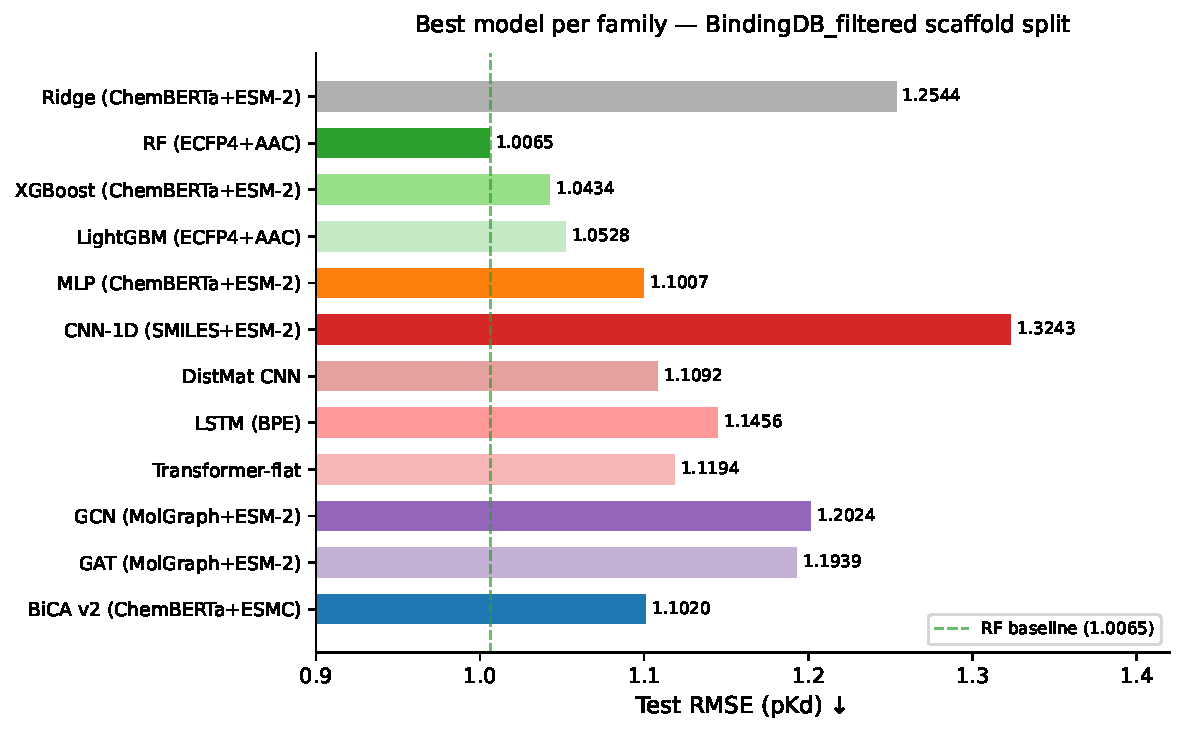
\includegraphics[width=0.95\linewidth]{../figures/fig1_leaderboard.pdf}
  \caption{\textbf{Benchmark leaderboard across 12 model families.}
    Bar chart of test-set RMSE for the best configuration in each model family
    (seed~42, Bemis--Murcko scaffold split).  Error bars for multi-seed models
    indicate the range across seeds~$\{42, 123, 456\}$.  RF denotes Random
    Forest; XGB, XGBoost; BiCA, Bidirectional Cross-Attention.  Colour
    indicates model type: grey = tree ensembles; blue = sequence models;
    orange = graph neural networks; green = attention/cross-attention.}
  \label{fig:leaderboard}
\end{figure}

\begin{figure}[htbp]
  \centering
  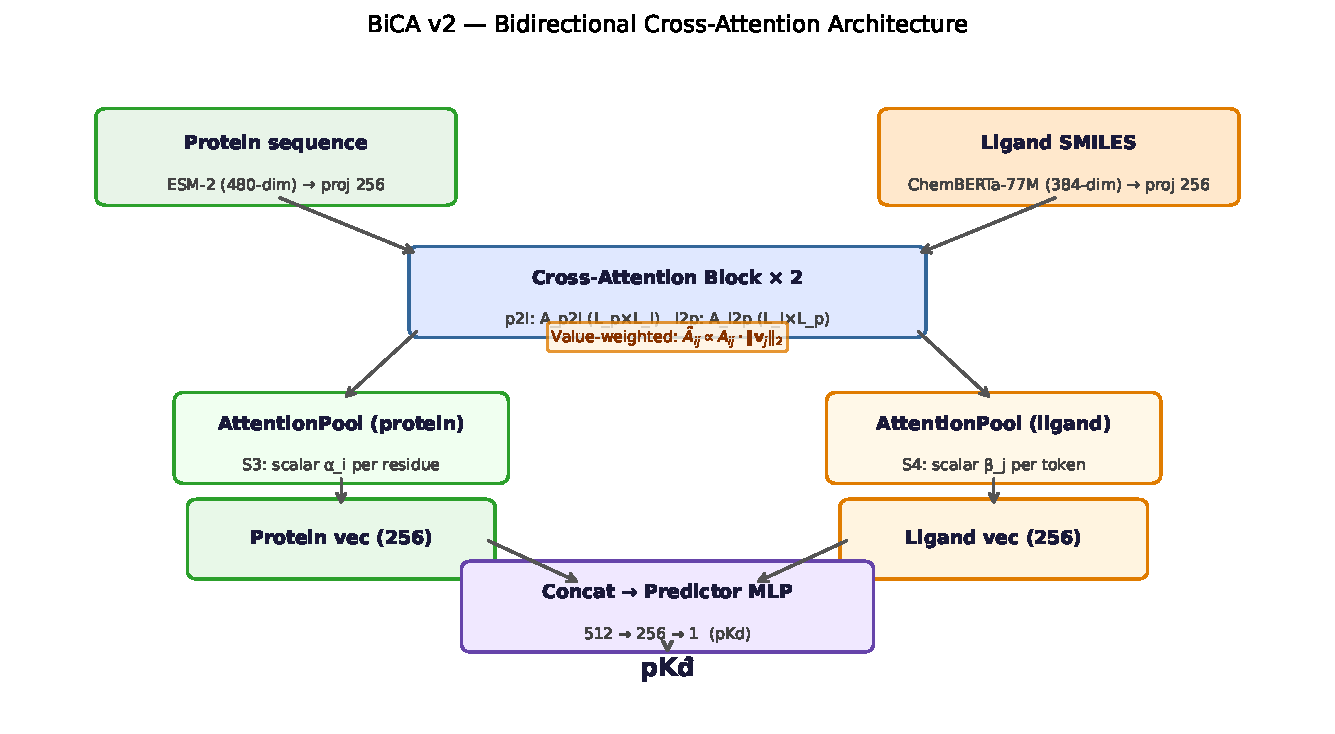
\includegraphics[width=0.95\linewidth]{../figures/fig2_architecture.pdf}
  \caption{\textbf{BiCA~v2 architecture.}
    Schematic of the Bidirectional Cross-Attention v2 model.  Per-residue
    ESM-2 embeddings and per-token ChemBERTa-2 embeddings are projected to a
    shared hidden dimension and passed through two stacked bidirectional
    cross-attention blocks (each with 8~heads and a position-wise FFN).
    Gated attention pooling reduces each sequence to a fixed vector; the
    pooled vectors are concatenated and passed to a three-layer MLP predictor.}
  \label{fig:bica_arch}
\end{figure}

\begin{figure}[htbp]
  \centering
  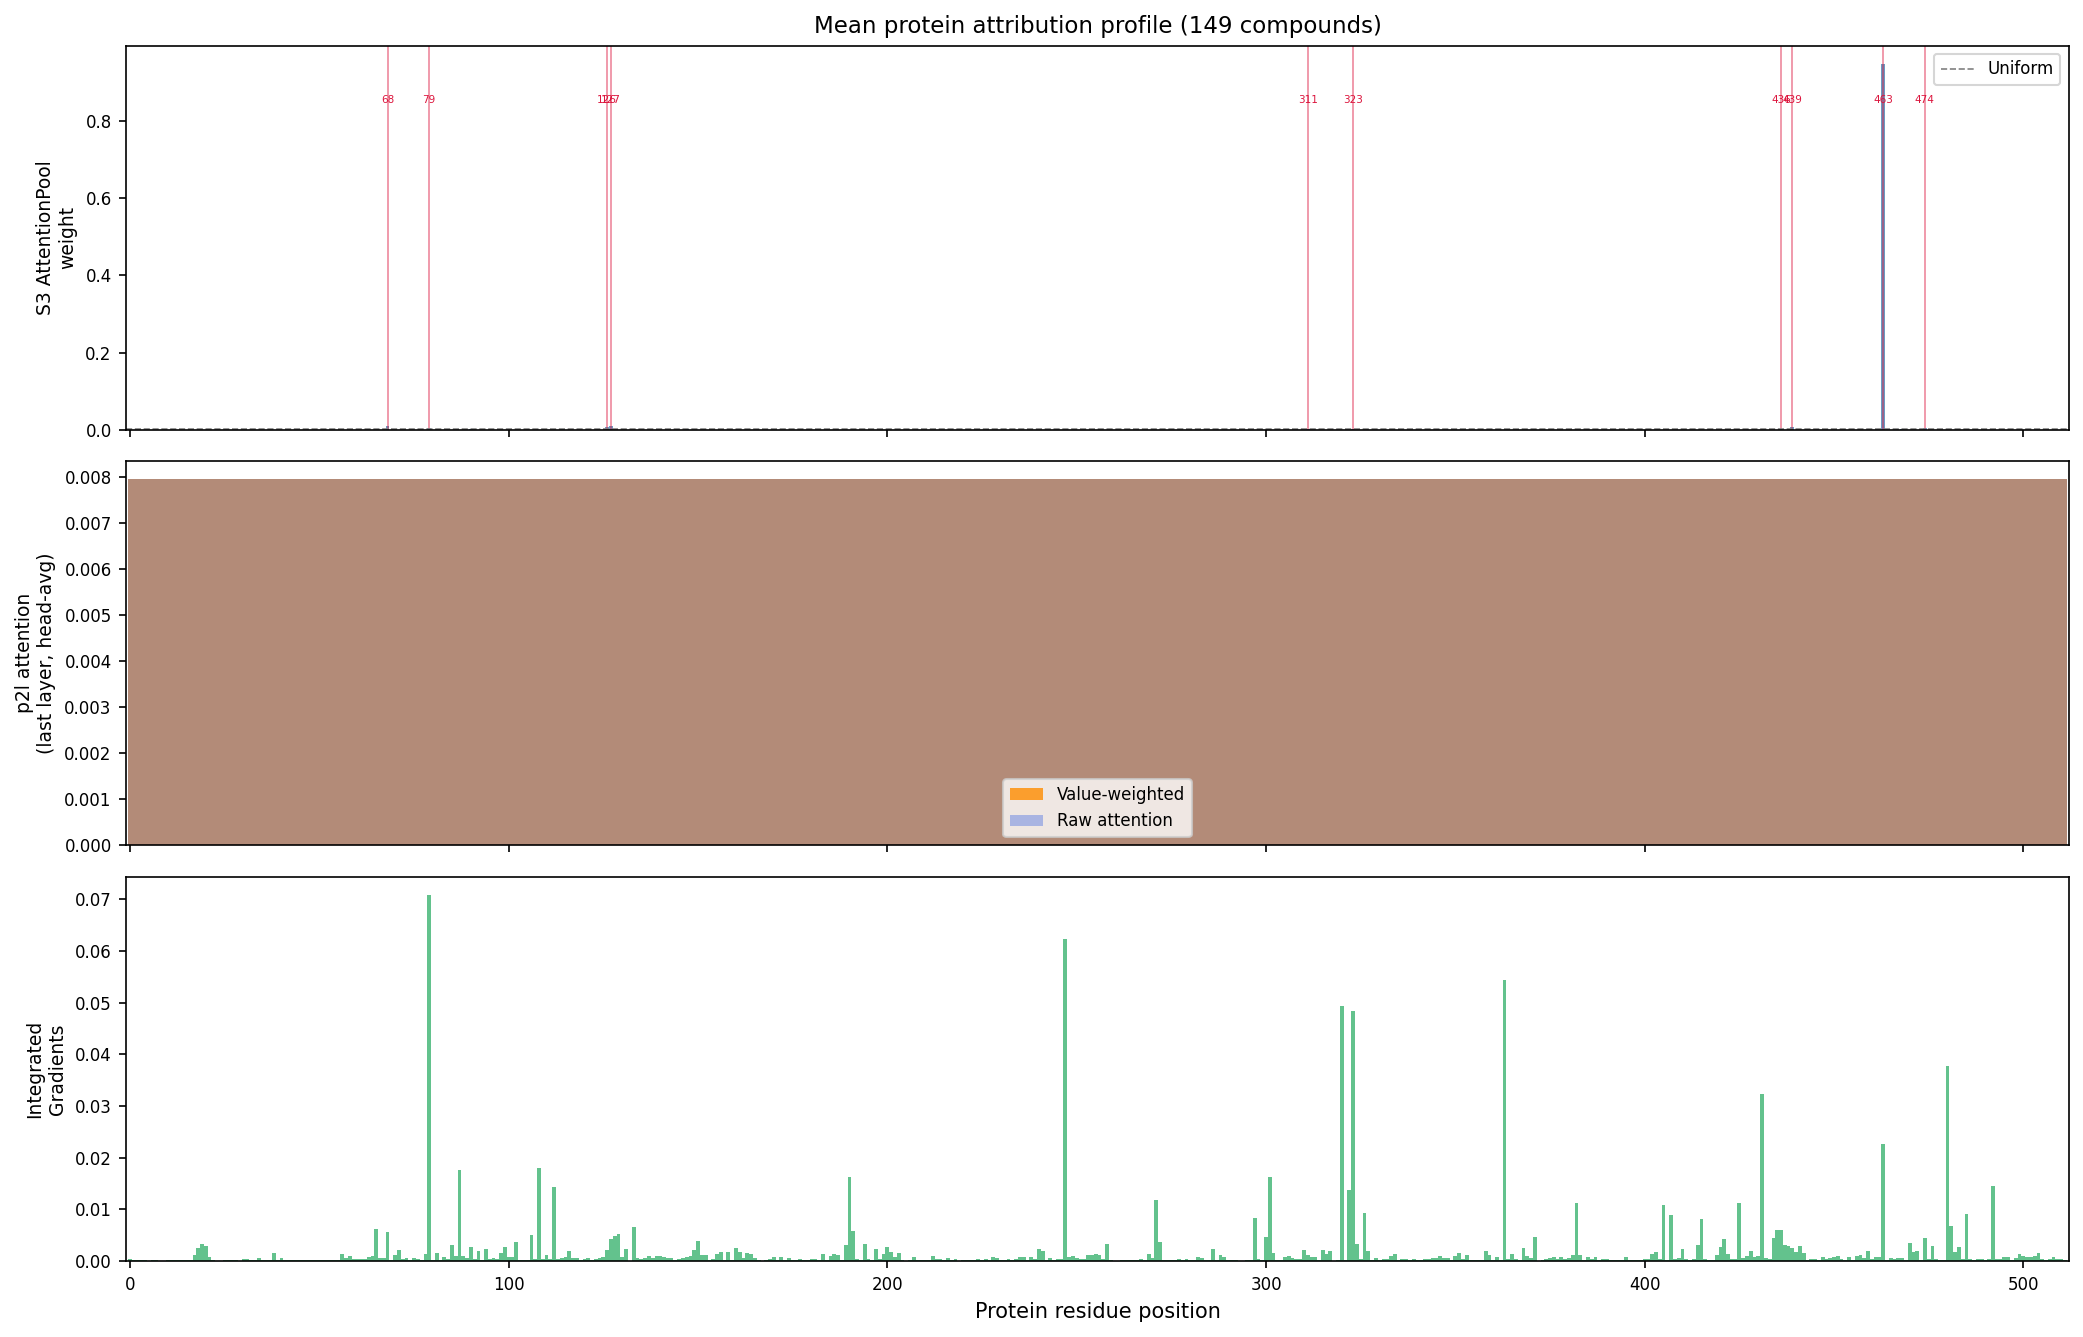
\includegraphics[width=0.95\linewidth]{../figures/fig3_protein_consensus.png}
  \caption{\textbf{Mean protein attribution profiles across 149 compounds.}
    Each panel shows the mean (across 149 test-set inhibitors of a 1130-aa
    kinase-like protein) of one attribution signal as a function of residue
    position (0-indexed, truncated to 512).  \textit{Top}: AttentionPool
    (S3) weights; the dashed line marks the uniform expectation $1/512$.
    Residue~463 (Cys, context \texttt{ERPEGCPEKVY}) carries $94.9\%$ of
    total weight.  \textit{Middle}: Head-averaged cross-attention p$\to$l
    (S1), raw (blue) vs value-weighted (orange).  \textit{Bottom}:
    Integrated Gradients attribution, normalised to sum to 1.  Vertical grey
    lines mark the five consensus residues (\{68, 79, 127, 323, 463\}).}
  \label{fig:protein_consensus}
\end{figure}

\begin{figure}[htbp]
  \centering
  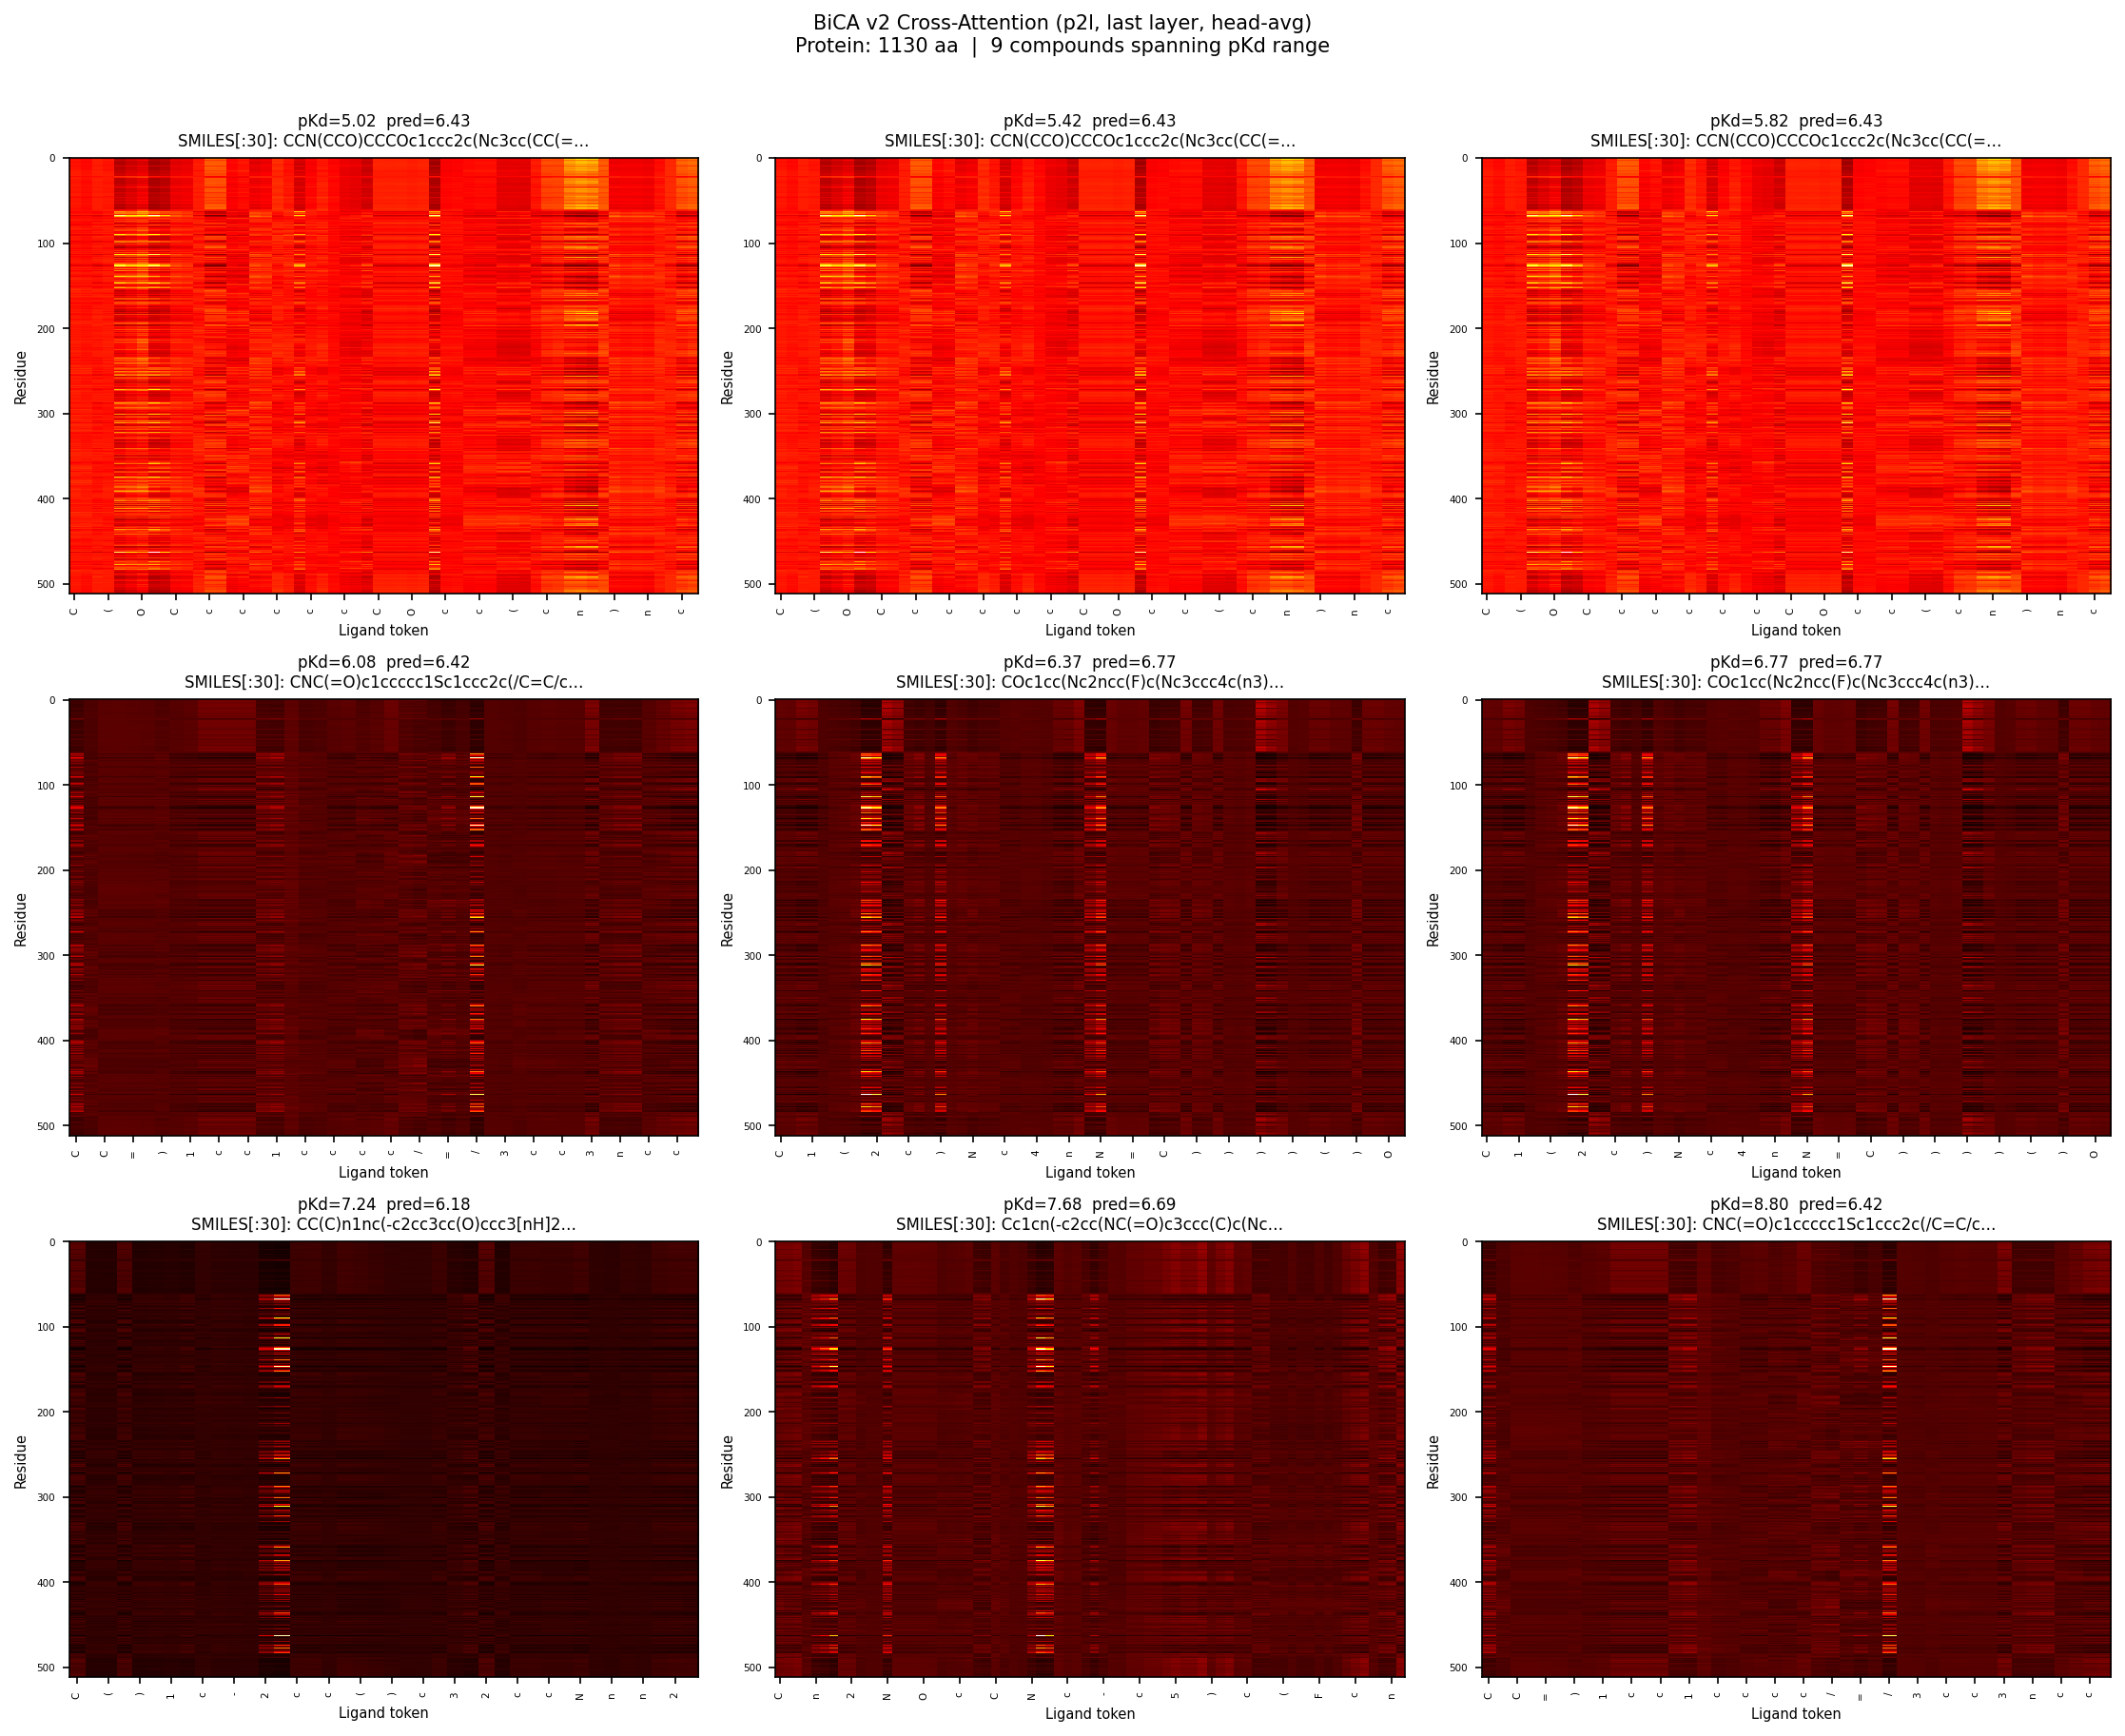
\includegraphics[width=\linewidth]{../figures/fig4_top_compounds_heatmap.png}
  \caption{\textbf{Residue~$\times$~token cross-attention heatmaps for nine
    compounds spanning the pKd range.}
    Each panel shows the head-averaged S1 cross-attention matrix (protein
    residues on the Y-axis; ChemBERTa tokens, decoded to SMILES substrings,
    on the X-axis) for one compound.  pKd and predicted pKd are indicated.
    Hot spots visible as horizontal bands (residues) and vertical stripes
    (ligand tokens) are consistent across compounds, confirming
    compound-independent protein-side attribution.}
  \label{fig:heatmaps}
\end{figure}

\begin{figure}[htbp]
  \centering
  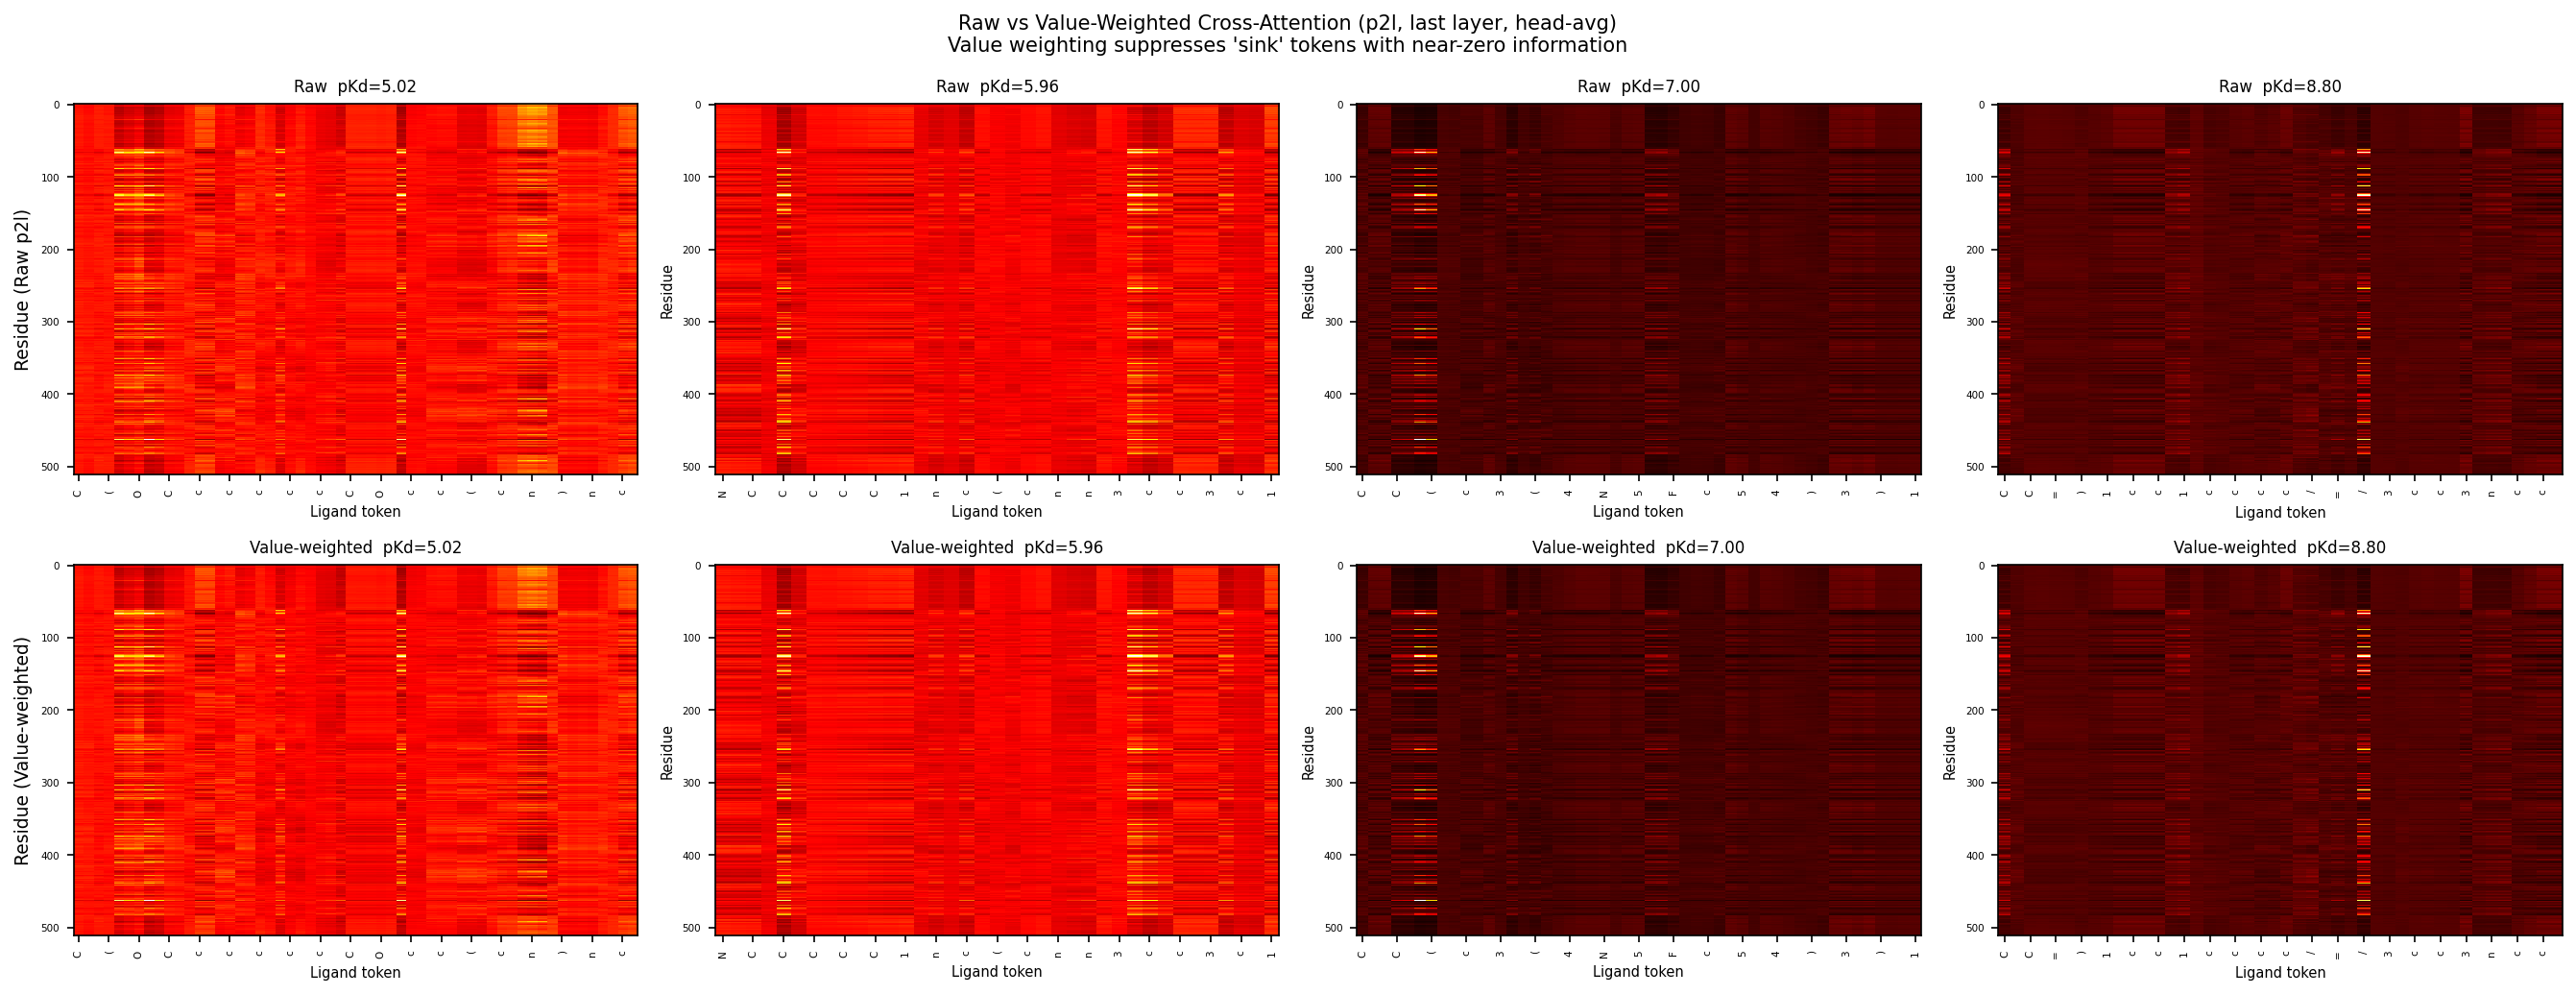
\includegraphics[width=0.95\linewidth]{../figures/fig5_value_weighted.png}
  \caption{\textbf{Value-weighted attention suppresses sink tokens.}
    Four representative compounds (columns) spanning the pKd range.
    \textit{Top row}: Raw cross-attention (S1, head-averaged).
    \textit{Bottom row}: Value-weighted cross-attention.  The value-weighted
    maps show sparser, more compound-specific ligand token patterns, while
    raw maps include high-weight positions that carry near-zero Value vector
    norms (``sink tokens'').}
  \label{fig:vw_comparison}
\end{figure}

\begin{figure}[htbp]
  \centering
  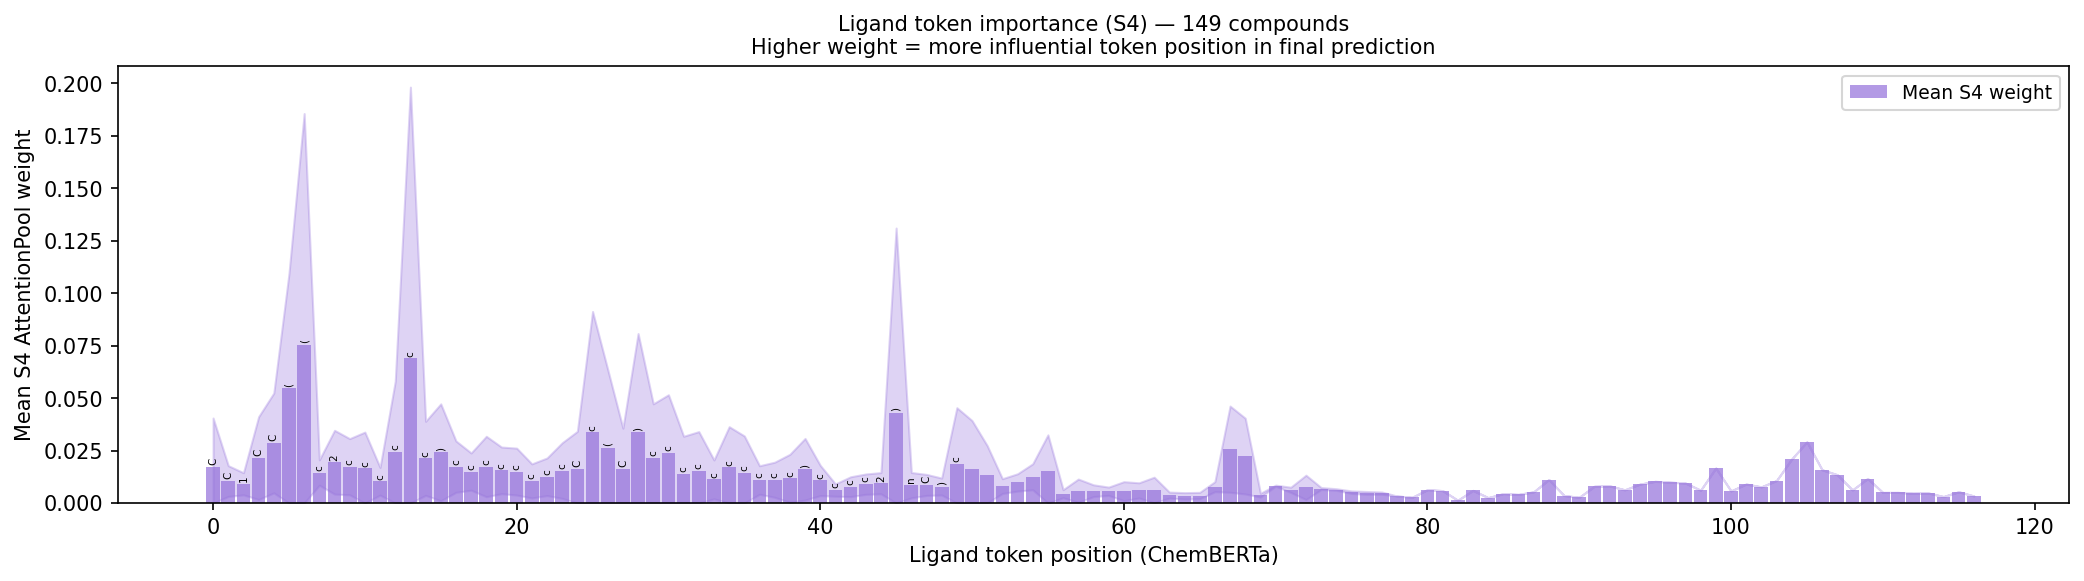
\includegraphics[width=0.9\linewidth]{../figures/fig6_token_importance.png}
  \caption{\textbf{Ligand token importance (S4 AttentionPool).}
    Mean S4~AttentionPool weight as a function of ChemBERTa token position
    across 149~compounds.  Shading indicates~$\pm 1$~standard deviation.
    Token labels at positions 0--15 (decoded from the most frequent token at
    each position across compounds) are shown above bars.  Weight
    concentrates on positions~$\lesssim 15$, corresponding to ring-core and
    early heteroatom tokens.}
  \label{fig:token_importance}
\end{figure}

\begin{figure}[htbp]
  \centering
  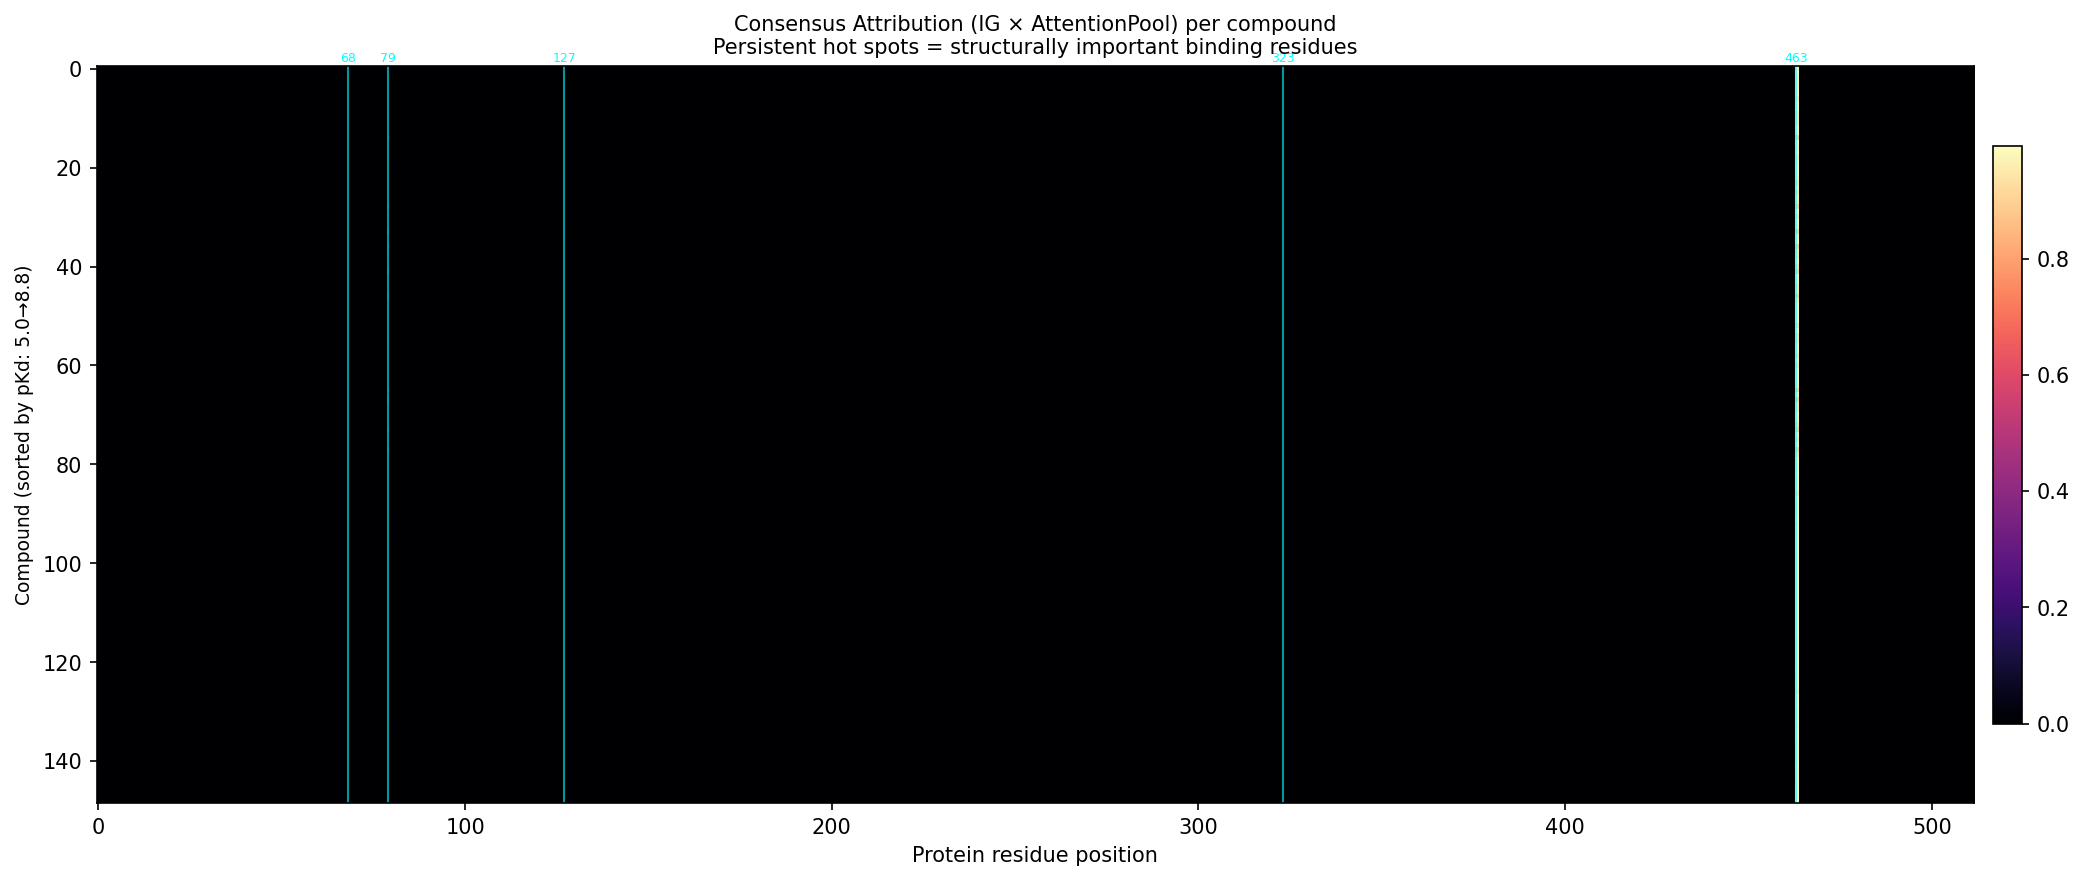
\includegraphics[width=0.9\linewidth]{../figures/fig7_consensus_heatmap.png}
  \caption{\textbf{Consensus attribution matrix.}
    Consensus score $c_i = \alpha_i^{(\text{IG})} \cdot w_i^{(\text{S3})}$
    for each compound (rows, sorted by increasing pKd) and residue position
    (columns).  Persistent hot spots are visible as vertical bright stripes,
    dominated by position~463.  Cyan vertical lines and labels mark the
    five consensus residues identified by mean $c_i$.}
  \label{fig:consensus}
\end{figure}

\end{document}
